% cSpell:ignore CMOS,TTL,7413,74121,74122,74123,555,VDD,VTH,VOH,VOL,Tplus,Tminus,TR,TF,TW,RC,EXT,TRIG,THRESH,DISCH,Crystal,VCES,VIK
\setlength{\parskip}{0.4em}
\setlength{\itemsep}{0.2em}
\setlength{\tabcolsep}{4pt}

\chapter{脉冲波形的产生和整形电路}
\section{概述}
\subsection{获取矩形脉冲的两条途径}
\begin{enumerate}
    \item \textbf{产生}：用各种形式的多谐振荡器直接产生矩形脉冲，不需要外加触发信号；
    \item \textbf{整形}：用整形电路（施密特触发器、单稳态触发器）把已有的周期性波形变换成符合要求的矩形脉冲。
\end{enumerate}
四类电路的分工：\textbf{施密特触发器}做整形与鉴幅；\textbf{单稳态触发器}做定时（把任意宽度输入变成固定宽度输出）；
\textbf{多谐振荡器}做振荡源；\textbf{555 定时器}则把这三类电路统一在一片数模混合集成电路中实现。

\subsection{矩形脉冲的参数}
工程上用一组参数描述非理想矩形脉冲，各参数的定义都是"约定"，必须记准基准点。
\begin{table}[htbp]
\centering
\caption{矩形脉冲的参数定义}
\begin{tabular}{lll}
\toprule
参数 & 符号 & 定义 \\
\midrule
脉冲周期 & $T$ & 信号变化一次所需的时间 \\
脉冲频率 & $f$ & 单位时间内信号变化的次数，$f=1/T$ \\
脉冲幅度 & $V_\text{m}$ & 脉冲电压的最大变化幅度 \\
脉冲宽度 & $t_\text{W}$ & 从前沿 $0.5V_\text{m}$ 到后沿 $0.5V_\text{m}$ 的一段时间 \\
上升时间 & $t_\text{r}$ & 上升沿从 $0.1V_\text{m}$ 上升到 $0.9V_\text{m}$ 所需时间 \\
下降时间 & $t_\text{f}$ & 下降沿从 $0.9V_\text{m}$ 下降到 $0.1V_\text{m}$ 所需时间 \\
占空比 & $q$ & 脉冲宽度与周期的比值，$q=t_\text{W}/T$ \\
\bottomrule
\end{tabular}
\end{table}
\textbf{易错点}：$t_\text{W}$ 的基准是 $0.5V_\text{m}$，$t_\text{r}$、$t_\text{f}$ 的基准是 $0.1V_\text{m}$ 与 $0.9V_\text{m}$，三者不能混用；
把 $t_\text{W}$ 当成"两个 $0.9V_\text{m}$ 点之间的宽度"是本章最常见的估算错误。$q$ 只对周期性重复脉冲有意义。

\section{施密特触发器}
\subsection{晶体管施密特电路的结构与工作原理}
\paragraph{电路组成}
$T_1$、$T_2$ 是两只直接耦合的共射放大管：$T_1$ 集电极经 $R_1$ 接 $V_\text{CC}$，并直接送到 $T_2$ 基极；
$T_2$ 集电极经 $R_2$ 接 $V_\text{CC}$，该点即输出端 $v_O$；两管发射极接在公共发射极电阻 $R_\text{E}$ 上再接地。
课件取 $R_1=2\,\mathrm{k}\Omega$、$R_2=1.4\,\mathrm{k}\Omega$、$R_\text{E}=480\,\Omega$，输入 $v_I$ 加在 $T_1$ 基极。
\textbf{$R_\text{E}$ 由两管共用是本电路的核心}：任一管电流变化都会改变射极电位，从而改变另一管的 $v_\text{BE}$，
形成正反馈，使电路一旦被推动就迅速翻转，这就是回差与陡峭边沿的来源。

\paragraph{两个稳态}
\begin{enumerate}
    \item $v_I=0$ 时 $T_1$ 截止、$T_2$ 饱和，$v_O=V_\text{OL}$，此时
    $V_{\text{E}2}\approx\left(V_\text{CC}-V_\text{CES2}\right)\dfrac{R_\text{E}}{R_2+R_\text{E}}$；
    \item $v_I$ 为高电平时 $T_1$ 饱和、$T_2$ 截止，$v_O=V_\text{OH}$，此时
    $V_{\text{E}1}\approx\left(V_\text{CC}-V_\text{CES1}\right)\dfrac{R_\text{E}}{R_1+R_\text{E}}$。
\end{enumerate}

\paragraph{翻转过程}
$v_I$ 升高到"射极电位 $+\,0.7\,\mathrm{V}$"时 $T_1$ 开始导通，正反馈链为
$v_I\uparrow\rightarrow i_{\text{C}1}\uparrow\rightarrow v_{\text{C}1}\downarrow\rightarrow i_{\text{C}2}\downarrow
\rightarrow v_\text{E}\downarrow\rightarrow v_{\text{BE}1}\uparrow$，
结果 $T_1$ 导通、$T_2$ 截止，$v_O$ 迅速跳变为 $V_\text{OH}$，射极电位由 $V_{\text{E}2}$ 降为 $V_{\text{E}1}$。
$v_I$ 下降到 $V_{\text{E}1}+0.7\,\mathrm{V}$ 以下时 $T_1$ 脱离饱和，正反馈方向相反，$T_1$ 截止、$T_2$ 导通，$v_O$ 跳变为 $V_\text{OL}$。

\paragraph{两个阈值与回差}
\textbf{正向阈值电压} $V_{\text{T}+}$：输入上升过程中使 $T_1$ 开始导通、状态发生转换的输入电压；
\textbf{负向阈值电压} $V_{\text{T}-}$：输入下降过程中使 $T_1$ 脱离饱和、状态发生转换的输入电压；
\textbf{回差电压} $\Delta V_\text{T}=\left|V_{\text{T}+}-V_{\text{T}-}\right|$。
两者分别由 $V_{\text{E}2}$、$V_{\text{E}1}$ 加上 $0.7\,\mathrm{V}$ 决定，因 $R_1>R_2$ 保证 $V_{\text{E}2}>V_{\text{E}1}$，故必有 $V_{\text{T}+}>V_{\text{T}-}$，回差为正。

\paragraph{缺点与改进}
$T_2$ 饱和时 $v_O=V_\text{OL}\approx V_\text{CC}\dfrac{R_\text{E}}{R_2+R_\text{E}}$，课件给出 $V_\text{OL}\approx1.9\,\mathrm{V}$，
远非标准逻辑低电平，不能直接驱动 TTL/CMOS 负载。改进办法是加电平偏移电路与推拉式输出级、输入端改与门结构，即集成施密特触发器 7413。

\subsection{用门电路组成的施密特触发器}
\paragraph{电路结构}
两级 CMOS 反相器 $G_1$、$G_2$ 串接，用分压电阻 $R_1$、$R_2$ 把输出端电压反馈到 $G_1$ 输入节点 $v_A$。
设 $V_\text{TH}=V_\text{DD}/2$、$V_\text{OH}=V_\text{DD}$、$V_\text{OL}=0$，且 $R_1<R_2$。

\paragraph{分析方法（线性电路 + 叠加原理）}
正反馈过程本身无法直接计算，只算\textbf{临界点}：翻转前一刻正反馈尚未建立，可把电路当线性电路，
用叠加原理求 $v_A$ 并令它等于 $V_\text{TH}$（忽略门电路输入电流与正反馈动态过程）：
\[
v_A=\frac{R_2}{R_1+R_2}v_I+\frac{R_1}{R_1+R_2}v_O
\]

\paragraph{两个阈值与回差}
$v_I$ 上升、翻转前 $v_O=V_\text{OL}\approx0$，令 $v_A=V_\text{TH}$ 得正向阈值
\[
V_{\text{T}+}=\left(1+\frac{R_1}{R_2}\right)V_\text{TH}
\]
$v_I$ 下降、翻转前 $v_O=V_\text{OH}=V_\text{DD}$，令 $v_A=V_\text{TH}$ 得负向阈值
\[
V_{\text{T}-}=\left(1-\frac{R_1}{R_2}\right)V_\text{TH}
\]
两者之差即回差电压
\[
\Delta V_\text{T}=V_{\text{T}+}-V_{\text{T}-}=\frac{2R_1}{R_2}V_\text{TH}
\]
调节 $R_1/R_2$ 可同时改变 $V_{\text{T}+}$、$V_{\text{T}-}$ 与 $\Delta V_\text{T}$，比值越大回差越大；电路可接成同相、反相两种输出特性。

\begin{figure}[htbp]
\centering
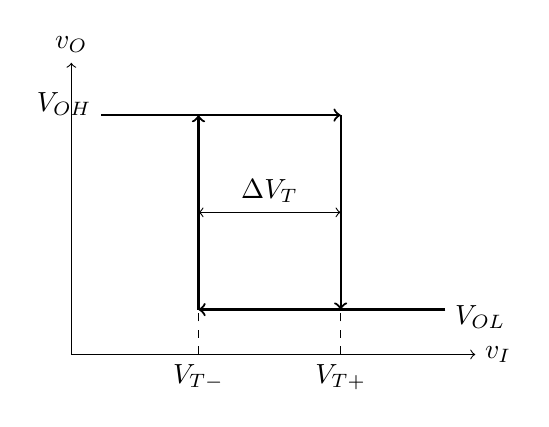
\begin{tikzpicture}[scale=0.95]
    \draw[->] (0,0) -- (5.4,0) node[right] {$v_I$};
    \draw[->] (0,0) -- (0,3.9) node[above] {$v_O$};
    % 滞回环：上支为 vI 增大时的路径，下支为 vI 减小时的路径
    \draw[thick,->] (0.4,3.2) -- (3.6,3.2);
    \draw[thick,->] (3.6,3.2) -- (3.6,0.6);
    \draw[thick,->] (5.0,0.6) -- (1.7,0.6);
    \draw[thick,->] (1.7,0.6) -- (1.7,3.2);
    \draw[dashed] (3.6,0) -- (3.6,0.6);
    \draw[dashed] (1.7,0) -- (1.7,0.6);
    \node[below] at (1.7,0) {$V_{\text{T}-}$};
    \node[below] at (3.6,0) {$V_{\text{T}+}$};
    \node[left] at (0.4,3.35) {$V_\text{OH}$};
    \node[right] at (5.0,0.5) {$V_\text{OL}$};
    \draw[<->] (1.7,1.9) -- (3.6,1.9);
    \node[above] at (2.65,1.9) {$\Delta V_\text{T}$};
\end{tikzpicture}
\caption{施密特触发器的电压传输特性（反相输出，箭头为 $v_I$ 变化方向）}
\end{figure}

\textbf{易错点}：两式只差一个符号，判据是"翻转前 $v_O$ 是什么电平"——$v_I$ 上升时翻转前 $v_O$ 为低电平，
反馈项使 $v_A$ 偏小，$v_I$ 必须更大，故 $V_{\text{T}+}$ 用 $1+R_1/R_2$；$v_I$ 下降时翻转前 $v_O$ 为高电平，
反馈项抬高 $v_A$，$v_I$ 可以更小，故 $V_{\text{T}-}$ 用 $1-R_1/R_2$。

\subsection{集成施密特触发器 7413}
7413 是 TTL 集成施密特触发器（双 4 输入与非门），内部四部分各有针对性：
\begin{enumerate}
    \item 输入级加"与门"，扩展输入端的逻辑功能；
    \item 施密特核心电路（正反馈回路），提供回差与陡峭边沿；
    \item 电平偏移电路，解决分立电路中 $V_\text{OL}$ 偏高的缺点；
    \item 推拉式输出级，使 $V_\text{OL}\le0.5\,\mathrm{V}$ 达到标准逻辑低电平，并提高带负载能力。
\end{enumerate}

\subsection{主要特点与典型应用}
\paragraph{主要特点}
输入信号在上升和下降过程中状态转换的输入电平不同（存在回差 $\Delta V_\text{T}$）；
状态转换时有正反馈，输出波形边沿变陡，与输入边沿陡缓无关；输入落在回差带内时输出保持原态，故抗噪声能力强。

\paragraph{典型应用}
\begin{enumerate}
    \item \textbf{波形变换}：把边沿缓慢的周期性信号（正弦、三角波）变为边沿很陡的矩形脉冲；
    \item \textbf{脉冲整形}：信号经长传输线（电容大、阻抗不匹配）或叠加噪声后变形，整形后得到理想波形；
    \item \textbf{脉冲鉴幅}：把幅度不同的脉冲序列中幅度大于 $V_{\text{T}+}$ 的脉冲鉴别出来，小于者被抑制。
\end{enumerate}

\section{单稳态触发器}
\subsection{电路特点}
\begin{enumerate}
    \item 有一个\textbf{稳态}和一个\textbf{暂稳态}；
    \item 在外界触发信号作用下由稳态翻到暂稳态，维持一段时间后\textbf{自动}返回稳态；
    \item 暂稳态时间只取决于\textbf{电路内部参数}（$R$、$C$），与触发脉冲的宽度、幅度无关。
\end{enumerate}
暂稳态靠 $RC$ 充放电维持，按 $RC$ 接法不同分为\textbf{微分型}与\textbf{积分型}。

\subsection{微分型单稳态触发器}
\paragraph{电路组成}
由 CMOS 门 $G_1$、$G_2$，输入端 $R_d$、$C_d$ 微分电路，以及接在 $G_1$ 输出与 $G_2$ 输入之间的 $R$、$C$ 定时电路组成。
设 $V_\text{OH}\approx V_\text{DD}$、$V_\text{OL}\approx0$、$V_\text{TH}\approx V_\text{DD}/2$。

\paragraph{工作过程}
\textbf{稳态}：无触发时 $v_I=0$、$v_{I2}=V_\text{DD}$，故 $v_O=0$、$v_{O1}=V_\text{DD}$，电容无电压 $v_C=0$。\\
\textbf{触发}：$v_I$ 加触发脉冲，$R_d$、$C_d$ 微分后得到很窄的正负尖峰 $v_d$；$v_d$ 升到 $V_\text{TH}$ 后产生正反馈
$v_d\uparrow\rightarrow v_{O1}\downarrow\rightarrow v_{I2}\downarrow\rightarrow v_O\uparrow$，
$v_{O1}$ 跳为低电平，电容电压不能跃变故 $v_{I2}$ 同时为低电平，$v_O$ 翻为高电平，进入暂稳态。\\
\textbf{返回}：暂稳态中 $V_\text{DD}$ 经 $R$ 和 $G_1$ 输出电路给 $C$ 充电，$v_{I2}$ 指数上升；到 $v_{I2}=V_\text{TH}$ 时又一次正反馈，
$v_{O1}$、$v_{I2}$ 跳回高电平，$v_O$ 回 0；随后 $C$ 经 $R$ 与 $G_2$ 输入保护电路迅速放电到 0，电路完全恢复。

\paragraph{脉冲宽度}
充电起始值 $v_C(0)=0$、终了值 $v_C(\infty)=V_\text{DD}$、转换值 $v_C(t_\text{W})=V_\text{TH}$，代入三要素公式
\[
t_\text{W}=\tau\ln\frac{v_C(\infty)-v_C(0)}{v_C(\infty)-v_C(t_\text{W})}
=RC\ln\frac{V_\text{DD}}{V_\text{DD}-V_\text{TH}}=RC\ln2\approx0.69RC
\]
严格写 $\tau\approx(R+R_\text{ON})C$，$R_\text{ON}$ 为 $G_1$ 导通时的输出电阻。

\paragraph{其余参数}
\[
T_\text{re}\approx(3\sim5)R_\text{ON}C,\qquad T_\text{d}=t_\text{W}+T_\text{re},\qquad V_\text{m}=V_\text{OH}-V_\text{OL}\approx V_\text{DD}
\]
$T_\text{re}$ 为恢复时间（经验公式），$T_\text{d}$ 为分辨时间，即相邻两次触发的最小间隔；脉冲周期取决于输入触发脉冲周期。
本电路可用窄脉冲触发，但输出脉冲的下降沿较差。

\subsection{积分型单稳态触发器}
\paragraph{电路组成与工作过程}
由 TTL 与非门、反相器和 $RC$ 积分电路组成，用\textbf{正脉冲}触发。
$v_I=0$ 为稳态，$v_{O1}=V_\text{OH}$ 经 $R$ 很快把 $C$ 充到 $v_A=V_\text{OH}$（$R$ 较小）。
$v_I$ 变高后 $v_{O1}=V_\text{OL}$，电容电压不能突变，$v_A$ 仍为高电平，$v_O=V_\text{OL}$，进入暂稳态，$C$ 经 $R$ 放电；
$v_A$ 降到 $G_2$ 开启电压 $V_\text{TH}$ 时输出翻回高电平，回到稳态；$v_I$ 回低电平后 $v_{O1}$ 重新为高并向 $C$ 充电。

\paragraph{脉冲宽度}
\[
t_\text{W}=(R+R_\text{O})C\ln\frac{V_\text{OL}-V_\text{OH}}{V_\text{OL}-V_\text{TH}}
\]
$R_\text{O}$ 为 $G_1$ 输出低电平时的输出电阻。

\subsection{两种单稳态触发器的比较}
\begin{table}[htbp]
\centering
\caption{微分型与积分型单稳态触发器的比较}
\begin{tabular}{lll}
\toprule
比较项 & 微分型 & 积分型 \\
\midrule
$RC$ 电路位置 & 门间耦合（微分） & $G_2$ 输入端（积分） \\
有无正反馈 & 有 & 无 \\
输出边沿 & 前后沿都比较陡 & 边沿较差 \\
抗干扰能力 & 差 & 强 \\
对触发脉冲的要求 & 可用窄脉冲（宽度小于 $t_\text{W}$） & 触发脉冲宽度必须大于 $t_\text{W}$ \\
\bottomrule
\end{tabular}
\end{table}

\subsection{集成单稳态触发器 74121}
\paragraph{引脚与触发方式}
$\overline{A_1}$、$\overline{A_2}$ 为\textbf{下降沿}触发端（两者至少一个接低电平），$B$ 为\textbf{上升沿}触发端；
片内设 $R_\text{int}\approx2\,\mathrm{k}\Omega$ 内部定时电阻可代替外接电阻，也可外接 $R_\text{ext}$、$C_\text{ext}$ 自行设定脉宽。

\paragraph{脉宽计算与范围}
\[
t_\text{W}=0.69R_\text{ext}C_\text{ext}
\]
课件适用范围：$R_\text{ext}=2\,\mathrm{k}\Omega\sim30\,\mathrm{k}\Omega$、$C_\text{ext}=10\,\mathrm{pF}\sim10\,\mu\mathrm{F}$，
对应 $t_\text{W}=20\,\mathrm{ns}\sim200\,\mathrm{ms}$。$R_\text{ext}$ 过小会损坏芯片，过大会因漏电流引入误差。

\paragraph{不可重复触发与可重复触发}
\textbf{不可重复触发型}：进入暂稳态后再加触发脉冲不影响工作过程，必须待暂稳态结束才能接受下一个触发，
74121、74221、74LS221 属此类；\textbf{可重复触发型}：暂稳态期间再次触发会重新计时，输出脉冲再延续一个 $t_\text{W}$
（脉宽被展宽），74122、74LS122、74123、74LS123 属此类；部分型号（74221、74122、74123）另设复位端可提前结束暂稳态。

\paragraph{应用}
\textbf{定时}：产生固定宽度的选通脉冲，宽度由 $R$、$C$ 精确设定而与输入无关；\textbf{整形}：把不规则输入整形成规范的宽度与幅度；
\textbf{延时}：用两级单稳的脉宽差实现脉冲延时输出。

\section{多谐振荡器}
\subsection{自激振荡的条件与分类}
多谐振荡器是\textbf{自激振荡器}，接通电源后不需外加触发信号即自动产生矩形脉冲；因矩形波含丰富高次谐波而得名（又称无稳态电路）。
自激振荡的必要条件是电路\textbf{没有稳定状态}，实现办法有两类：
\begin{enumerate}
    \item 让门电路静态时工作在电压传输特性的\textbf{转折区}（放大状态），任何微小扰动都被正反馈放大而振荡——对称式、非对称式；
    \item 利用\textbf{延迟负反馈}（门电路传输延迟加 $RC$ 延时）形成振荡——环形振荡器。
\end{enumerate}

\subsection{对称式多谐振荡器}
\paragraph{电路结构与静态工作点}
两反相器 $G_1$、$G_2$ 经耦合电容 $C_1$、$C_2$ 接成正反馈回路，并在各管输入与输出间跨接 $R_{F1}$、$R_{F2}$，
把静态工作点偏置到电压传输特性的转折区。忽略门输出电阻，由叠加定理得反馈电阻在输入端引入的电压
\[
v_I=\frac{R_F}{R_1+R_F}V_\text{CC}+\frac{R_1}{R_1+R_F}v_O
\]
该直线与电压传输特性的交点即静态工作点 $P$；只要 $P$ 落在转折区（电压放大倍数大于 1），电路必然振荡。
对 74 系列门，$R_F$ 约取 $0.5\sim1.9\,\mathrm{k}\Omega$。

\paragraph{振荡过程与周期}
扰动使 $v_{I1}$ 微升，经两级正反馈后 $v_{O1}$ 变低、$v_{O2}$ 变高，进入第一个暂稳态，同时 $C_1$ 充电、$C_2$ 放电；
$C_1$ 同时经 $R_1$ 与 $R_{F2}$ 两条支路充电，充电较快，$v_{I2}$ 先升到 $V_\text{TH}$，又触发一次正反馈，进入第二个暂稳态，如此往复。
把 $C_1$ 充电回路用戴维宁定理等效得 $R_{\text{E}1}=\dfrac{R_1R_{F2}}{R_1+R_{F2}}$、
$V_{\text{E}1}=V_\text{OH}+\dfrac{R_{F2}}{R_1+R_{F2}}\left(V_\text{CC}-V_\text{OH}-V_\text{BE}\right)$；
考虑 TTL 输入钳位二极管，负跳变只能下跳到 $V_\text{IK}$，故 $v_C(0)=V_\text{IK}$、$v_C(\infty)=V_{\text{E}1}$、$v_C(t)=V_\text{TH}$：
\[
T_1=R_{\text{E}1}C_1\ln\frac{V_{\text{E}1}-V_\text{IK}}{V_{\text{E}1}-V_\text{TH}},
\qquad
T=2T_1=2R_\text{E}C\ln\frac{V_\text{E}-V_\text{IK}}{V_\text{E}-V_\text{TH}}
\]
若为 74LS 系列（$V_\text{OH}=3.4\,\mathrm{V}$、$V_\text{IK}=-1\,\mathrm{V}$、$V_\text{TH}=1.1\,\mathrm{V}$）且 $R_F\ll R_1$，可简化为
\[
T\approx2R_FC\ln\frac{V_\text{OH}-V_\text{IK}}{V_\text{OH}-V_\text{TH}}\approx1.3R_FC
\]

\subsection{非对称式多谐振荡器}
\paragraph{简化思路}
对称式电路中 $G_1$ 静态时工作在转折区，其输出电压本身就是界于高、低电平之间的偏置电压，直接接到 $G_2$ 输入端
即可使 $G_2$ 的静态工作点也落在转折区，因此可去掉 $C_2$ 与 $R_{F2}$，只在反馈回路保留一只电容 $C$ 与电阻 $R_F$。

\paragraph{静态工作点与周期}
以 CMOS 反相器为例，$R_F$ 跨接在 $G_1$ 输入与输出间且 $G_1$ 输入电流近似为零，故 $v_{O1}=v_{I1}$，
该直线与电压传输特性的交点即静态工作点，又因 $v_{I2}=v_{O1}$，$G_2$ 的静态工作点也在特性中点；流过 $R_F$ 的静态电流近似为零，对 $R_F$ 阻值无严格限制。
设 $G_2$ 输入保护电阻 $R_S$ 足够大、$R_F$ 远大于门导通电阻，则
$T_1\approx R_FC\ln\dfrac{V_\text{DD}-V_{\text{T}-}}{V_\text{DD}-V_{\text{T}+}}\approx R_FC\ln3$，放电时间同理，故
\[
T=T_1+T_2=2R_FC\ln3\approx2.2R_FC
\]
这是本章出现频率最高的多谐振荡周期公式，务必记住系数 $2.2$ 与 $\ln3$。

\subsection{环形振荡器}
把奇数个（$n\ge3$）反相器首尾相连构成闭合回路，利用门电路\textbf{传输延迟时间}形成延迟负反馈即产生自激振荡。
静态时任一门的输入、输出都不可能稳定在高、低电平，只能处于放大状态，故电路无稳定状态；
扰动经 $n$ 级延迟 $n\,t_\text{pd}$ 反相回到起点，再经 $n\,t_\text{pd}$ 又反相一次，如此往复：
\[
T=2n\,t_\text{pd}
\]
$n$ 为串联反相器个数（奇数），$t_\text{pd}$ 为单级门平均传输延迟时间。
门电路延迟极短（TTL 几十纳秒、CMOS 一二百纳秒），基本环形电路频率高且不易调节；
实用电路在回路中串入 $RC$ 延迟环节（并在 $G_1$ 输入端加保护电阻），使周期主要由 $RC$ 决定、频率可连续调节。

\subsection{用施密特触发器构成的多谐振荡器}
\paragraph{工作原理}
施密特反相器输出经 $R$ 反馈到输入端，输入端再经 $C$ 接地。设通电时 $v_I=0$、$v_O=V_\text{OH}$，
$V_\text{OH}$ 经 $R$ 向 $C$ 充电使 $v_I$ 上升；到 $V_{\text{T}+}$ 时输出翻为 $V_\text{OL}$，$C$ 经 $R$ 放电使 $v_I$ 下降；
降到 $V_{\text{T}-}$ 时又翻回高电平，在 $V_{\text{T}-}$ 与 $V_{\text{T}+}$ 之间往复振荡。

\paragraph{振荡周期与占空比调节}
设 CMOS 施密特触发器 $V_\text{OL}\approx0$、$V_\text{OH}\approx V_\text{DD}$，则
\[
T=RC\ln\left(\frac{V_\text{DD}-V_{\text{T}-}}{V_\text{DD}-V_{\text{T}+}}\cdot\frac{V_{\text{T}+}}{V_{\text{T}-}}\right)
\]
第一项对应充电时间、第二项对应放电时间。基本电路占空比不可调；
若在充电、放电支路各串一只方向相反的二极管，使充电只经 $R_2$、放电只经 $R_1$，则
\[
T=T_1+T_2\approx R_2C\ln\frac{V_\text{DD}-V_{\text{T}-}}{V_\text{DD}-V_{\text{T}+}}
+R_1C\ln\frac{V_{\text{T}+}}{V_{\text{T}-}}
\]
改变 $R_1$、$R_2$ 的比值即可改变占空比。

\subsection{石英晶体多谐振荡器}
石英晶体在固有谐振频率 $f_0$ 处阻抗最小（接近纯电阻）、相移为零，满足振荡的相位条件；偏离 $f_0$ 时阻抗迅速增大，
正反馈不足以维持振荡。故把晶体串入反馈回路后，\textbf{振荡频率只取决于晶体的固有谐振频率}，与 $R$、$C$ 及电源电压几乎无关。
典型电路用反相器配晶体与两只约 $30\,\mathrm{pF}$ 的匹配电容，频率稳定度可达 $10^{-5}\sim10^{-6}$ 量级，
远高于 $RC$ 型多谐振荡器（约 $10^{-1}\sim10^{-2}$），常用于时钟基准与时基电路。
晶体既可接在对称式、也可接在非对称式多谐振荡电路中，两者振荡频率都由晶体决定，$RC$ 只影响起振与输出波形。

\section{555 定时器及其应用}
\subsection{电路结构与功能表}
\paragraph{内部组成}
555 是数/模混合集成电路，由五部分组成：
\begin{enumerate}
    \item 三个 $5\,\mathrm{k}\Omega$ 电阻构成分压器，为比较器提供 $\frac{2}{3}V_\text{CC}$ 与 $\frac{1}{3}V_\text{CC}$ 的参考电压；
    \item 电压比较器 $C_1$、$C_2$：$C_1$ 反相端接高电平触发端 TH（6 脚）、同相端接 $\frac{2}{3}V_\text{CC}$；
    $C_2$ 同相端接低电平触发端 $\overline{\text{TR}}$（2 脚）、反相端接 $\frac{1}{3}V_\text{CC}$；
    \item SR 锁存器，把两比较器输出锁存为 $Q$、$\overline{Q}$；
    \item 输出缓冲器 $G$，输出端（3 脚）电流可达 $200\,\mathrm{mA}$；
    \item 放电三极管 $T_D$（OC 输出管），受 $\overline{Q}$ 控制，$Q=0$ 时导通，外接电容经 7 脚放电。
\end{enumerate}

\paragraph{功能表}
\begin{table}[htbp]
\centering
\caption{555 定时器的功能表（CB555）}
\begin{tabular}{ccccc}
\toprule
$\overline{R_D}$ & $v_{I1}$（TH，6 脚） & $v_{I2}$（$\overline{\text{TR}}$，2 脚） & $v_O$ & $T_D$ \\
\midrule
0 & $\times$ & $\times$ & 低 & 导通 \\
1 & $>\frac{2}{3}V_\text{CC}$ & $>\frac{1}{3}V_\text{CC}$ & 低 & 导通 \\
1 & $<\frac{2}{3}V_\text{CC}$ & $>\frac{1}{3}V_\text{CC}$ & 不变 & 不变 \\
1 & $<\frac{2}{3}V_\text{CC}$ & $<\frac{1}{3}V_\text{CC}$ & 高 & 截止 \\
1 & $>\frac{2}{3}V_\text{CC}$ & $<\frac{1}{3}V_\text{CC}$ & 高 & 截止 \\
\bottomrule
\end{tabular}
\end{table}
记忆口诀：\textbf{"都大为 0，都小为 1，一小一大是保持"}；$\overline{R_D}=0$ 时无条件复位。

\paragraph{各引脚功能}
1 脚接地 GND；2 脚低电平触发端（$v_{I2}<\frac{1}{3}V_\text{CC}$ 使 $Q=1$）；3 脚输出端（输出电压约比电源低 $1\sim3\,\mathrm{V}$，
可直接驱动继电器、LED、扬声器）；4 脚复位端 $\overline{R_D}$（输入负脉冲直接复位，不用时接高电平）；
5 脚电压控制端 $V_\text{CO}$（外加电压可改变比较器参考电压，不用时悬空或经 $0.01\,\mu\mathrm{F}$ 电容接地）；
6 脚高电平触发端 TH（$v_{I1}>\frac{2}{3}V_\text{CC}$ 使 $Q=0$）；7 脚放电端（$Q=0$ 时 $T_D$ 导通，外接电容经此放电）；
8 脚电源端（$5\sim18\,\mathrm{V}$）。

\subsection{接成施密特触发器}
\paragraph{接法与阈值}
2、6 脚短接作输入端，4、8 脚接电源，5 脚经 $0.01\,\mu\mathrm{F}$ 电容接地，7 脚悬空。
$v_I$ 升高：$v_I<\frac{1}{3}V_\text{CC}$ 时 $Q=1$、$v_O=V_\text{OH}$；$\frac{1}{3}V_\text{CC}<v_I<\frac{2}{3}V_\text{CC}$ 时保持；
$v_I>\frac{2}{3}V_\text{CC}$ 时 $Q=0$、$v_O=V_\text{OL}$。故 $V_{\text{T}+}=\frac{2}{3}V_\text{CC}$。
$v_I$ 降低：$v_I<\frac{1}{3}V_\text{CC}$ 时 $Q=1$、$v_O=V_\text{OH}$。故 $V_{\text{T}-}=\frac{1}{3}V_\text{CC}$，回差 $\Delta V_\text{T}=\frac{1}{3}V_\text{CC}$。

\paragraph{回差可调}
若 5 脚由外电路提供 $V_\text{CO}$，则 $V_{\text{T}+}=V_\text{CO}$、$V_{\text{T}-}=\frac{1}{2}V_\text{CO}$、$\Delta V_\text{T}=\frac{1}{2}V_\text{CO}$，
改变 5 脚电压即可任意调节阈值与回差，这是 555 相对集成施密特触发器的优势。

\subsection{接成单稳态触发器}
\paragraph{接法与工作过程}
2 脚作触发输入，6、7 脚短接后接 $RC$ 定时回路（$R$ 接 $V_\text{CC}$、$C$ 接地），5 脚经 $0.01\,\mu\mathrm{F}$ 电容接地。
\textbf{稳态}：无触发时 $v_{I2}>\frac{1}{3}V_\text{CC}$，若通电后 $Q=0$，则 $T_D$ 导通、$C$ 经 7 脚放电到 $v_C=0$，
$v_{I1}=0<\frac{2}{3}V_\text{CC}$，锁存器保持 $Q=0$、$v_O=0$。
\textbf{暂稳态}：触发脉冲下降沿使 $v_{I2}<\frac{1}{3}V_\text{CC}$，锁存器置 1，$Q=1$、$v_O$ 跳高、$T_D$ 截止，
$V_\text{CC}$ 经 $R$ 给 $C$ 充电；$v_C$ 充到 $\frac{2}{3}V_\text{CC}$ 时 $C_1$ 使锁存器复位，$Q=0$、$v_O$ 回低、$T_D$ 导通，$C$ 迅速放电，恢复稳态。

\paragraph{脉宽计算}
充电起始值 $v_C(0)=0$、终了值 $v_C(\infty)=V_\text{CC}$、转换值 $v_C(t_\text{W})=\frac{2}{3}V_\text{CC}$：
\[
t_\text{W}=RC\ln\frac{V_\text{CC}-0}{V_\text{CC}-\frac{2}{3}V_\text{CC}}=RC\ln3\approx1.1RC
\]
\textbf{易错点}：555 单稳系数是 $1.1$（$\ln3$），门电路微分型单稳是 $0.69$（$\ln2$），不可混用；
差别源于充电的"目标值"不同——前者充到 $\frac{2}{3}V_\text{CC}$ 就翻转，后者充到 $\frac{1}{2}V_\text{DD}$ 就翻转。
此外触发脉冲宽度必须小于 $t_\text{W}$、幅度应低于 $\frac{1}{3}V_\text{CC}$，否则电路无法正常返回。

\subsection{接成多谐振荡器}
\paragraph{接法与工作过程}
2、6 脚短接后接电容 $C$ 上端（$C$ 下端接地）；7 脚接在 $R_1$、$R_2$ 之间，$R_1$ 另一端接 $V_\text{CC}$、$R_2$ 另一端接 2、6 脚。
设通电后 $Q=1$、$T_D$ 截止，$V_\text{CC}$ 经 $R_1$、$R_2$ 给 $C$ 充电，$v_C$ 上升；到 $\frac{2}{3}V_\text{CC}$ 时 $C_1$ 使锁存器复位，
$Q=0$、$T_D$ 导通，$C$ 经 $R_2$ 与 $T_D$ 放电，$v_C$ 下降；到 $\frac{1}{3}V_\text{CC}$ 时 $C_2$ 使锁存器置 1，$T_D$ 又截止，重新充电，
在 $\frac{1}{3}V_\text{CC}$ 与 $\frac{2}{3}V_\text{CC}$ 之间往复，输出连续矩形波。

\paragraph{周期与占空比}
\[
T_1=(R_1+R_2)C\ln2,\quad T_2=R_2C\ln2,\quad
T=(R_1+2R_2)C\ln2\approx0.69(R_1+2R_2)C
\]
\[
q=\frac{T_1}{T}=\frac{R_1+R_2}{R_1+2R_2}>50\%
\]
标准 555 多谐振荡器的占空比恒大于 50\%、不能小于 50\%，这是其固有缺点。

\paragraph{占空比可调的改进电路}
在 $R_1$、$R_2$ 支路各串一只方向相反的二极管，使充电只经 $R_\text{充}$、放电只经 $R_\text{放}$，则
\[
T_1=R_\text{充}C\ln2,\quad T_2=R_\text{放}C\ln2,\quad
T=(R_\text{充}+R_\text{放})C\ln2,\quad q=\frac{R_\text{充}}{R_\text{充}+R_\text{放}}
\]
选取不同的 $R_\text{充}$、$R_\text{放}$ 即可得到任意占空比（包括小于 50\%）。

\section{本章分析步骤与易错点}
\subsection{三类电路的分析步骤}
\begin{enumerate}
    \item \textbf{施密特触发器}：判断两个稳态（谁导通、$v_O$ 为何电平）→ 找翻转的临界条件（$v_A=V_\text{TH}$ 或 $v_I=v_\text{E}+0.7\,\mathrm{V}$）
    → 用叠加原理或分压关系解出 $V_{\text{T}+}$、$V_{\text{T}-}$ → 回差取两者之差。
    \item \textbf{单稳态触发器}：定稳态 → 定触发方式（上升沿/下降沿、哪一个端子）→ 定暂稳态由哪个 $RC$ 充放电维持
    → 用三要素公式求 $t_\text{W}$ → 校核恢复时间 $T_\text{re}$ 与分辨时间 $T_\text{d}$。
    \item \textbf{多谐振荡器}：找两个暂稳态的转换阈值 → 定每段充放电回路的等效电阻与等效电源 → 分别求 $T_1$、$T_2$
    → 相加得 $T$，占空比 $q=T_1/T$。
\end{enumerate}

\subsection{易错点清单}
\begin{itemize}
    \item $t_\text{W}=1.1RC$（$\ln3$）只属于"充到 $\frac{2}{3}V_\text{CC}$ 翻转"的场合（555 单稳、555 多谐的每一段）；
    门电路单稳与施密特型多谐的阈值是 $V_\text{TH}=V_\text{DD}/2$，对应 $\ln2\approx0.69$。
    \item 施密特触发器 $V_{\text{T}+}$、$V_{\text{T}-}$ 的反馈电平判断错，会导致回差符号反、甚至算出负回差。
    \item 555 的 5 脚接外参考 $V_\text{CO}$ 后，两个阈值变为 $V_\text{CO}$ 与 $V_\text{CO}/2$，不再是 $\frac{2}{3}V_\text{CC}$ 与 $\frac{1}{3}V_\text{CC}$。
    \item 标准 555 多谐振荡器的 $q$ 恒大于 50\%，不能靠改变 $R_1$、$R_2$ 的数值得到 $q<50\%$，必须改接二极管。
    \item 单稳态输出脉宽由 $R$、$C$ 决定而与触发脉冲无关；积分型单稳却要求触发脉冲宽度大于输出脉宽——
    这两句不矛盾：前者说"输出与输入无关"，后者说"电路正常工作的输入条件"。
\end{itemize}
